\chapter{Расчёт}

\section{Задание}
Произвести расчёт параметров контурного заземляющего устройства для защитного заземления электроустановок по следующим исходным данным: заземлители – стальные уголки с шириной полки $50$ мм, длиной $2.$6 м забиваются в землю на глубину $0.6$ м от ее поверхности; соединительная полоса – стальная труба шириной 40 мм; грунт – глина, удельное сопротивление которой $\rho = 60 \text{ Ом} \cdot \text{м}$. Расстояние между двумя соседними заземлителями $4$ м; значения коэффициентов: $K_\text{сез}  = 1.2$; $\eta_\text{з} = 0.6$; $\eta_\text{п} = 0.3$.

\section{Решение}

Определяется сопротивление растеканию тока в земле одного вертикального заземлителя $R_0$ в виде уголка, вбитого в землю ниже уровня ее поверхности.
\[
t = h + \frac{l_0}{2}= 0.6 + \frac{2.6}{2} = 1.9
\]

\[
\rho_\text{р} = \rho \cdot K_\text{сез} = 60 \cdot 1.2 = 72
\]

\begin{multline*}
R_\text{уг} = \frac{\rho_\text{р}}{2 \pi \cdot l_0} \cdot \left( \ln \frac{4 \cdot l_0}{0.95 \cdot b_\text{пу}} + \frac{1}{2} \ln \frac{4\cdot t +l_0}{4\cdot t -l_0} \right) =\\= \frac{72}{2\pi \cdot 2.6} \cdot \left(\ln \frac{4 \cdot 2.6}{0.95 \cdot 0.06} + \frac{1}{2} \ln \frac{4 \cdot 1.9 + 2.6}{4 \cdot 1.9 -2.6} \right) = 24.518
\end{multline*}

Определяем необходимое число вертикальных заземлителей $n$:
\[
n = \frac{R_\text{уг}}{R_\text{з}\cdot \eta_\text{з}} = \frac{24.518}{4 \cdot 0.6} = 10.215 \approx 10
\]

Рассчитываем длину соединительной полосы $l$:

\[
l = 1.05 \cdot a \cdot n = 1.05 \cdot 4 \cdot 10 = 42
\]

Определяем сопротивление соединительной полосы растеканию тока

\[
R_\text{п} = \frac{\rho_\text{р}}{2\pi \cdot l} \cdot \ln \frac{l^2}{d_\text{тр} \cdot h} = \frac{72}{2\pi \cdot 42} \cdot \ln \frac{42^2}{0.06 \cdot 0.6} = 2.996
\]

Рассчитываем полное сопротивление заземляющего устройства

\[
R_\text{зу} = \frac{R_\text{уг} \cdot R_\text{п}}{R_\text{уг} \cdot \eta_\text{п} + n\cdot R_\text{п} \cdot \eta_\text{з}}= \frac{24.518 \cdot 2.996}{24.518 \cdot 0.3 + 10 \cdot 2.996 \cdot 0.6} = 2.889
\]

Расчёт считаем законченным, так как сопротивление проектируемого заземляющего устройства менее 4 Ом, что соответствует требованиям ПУЭ.

\section{Схемы}

\begin{figure}
	\centering
	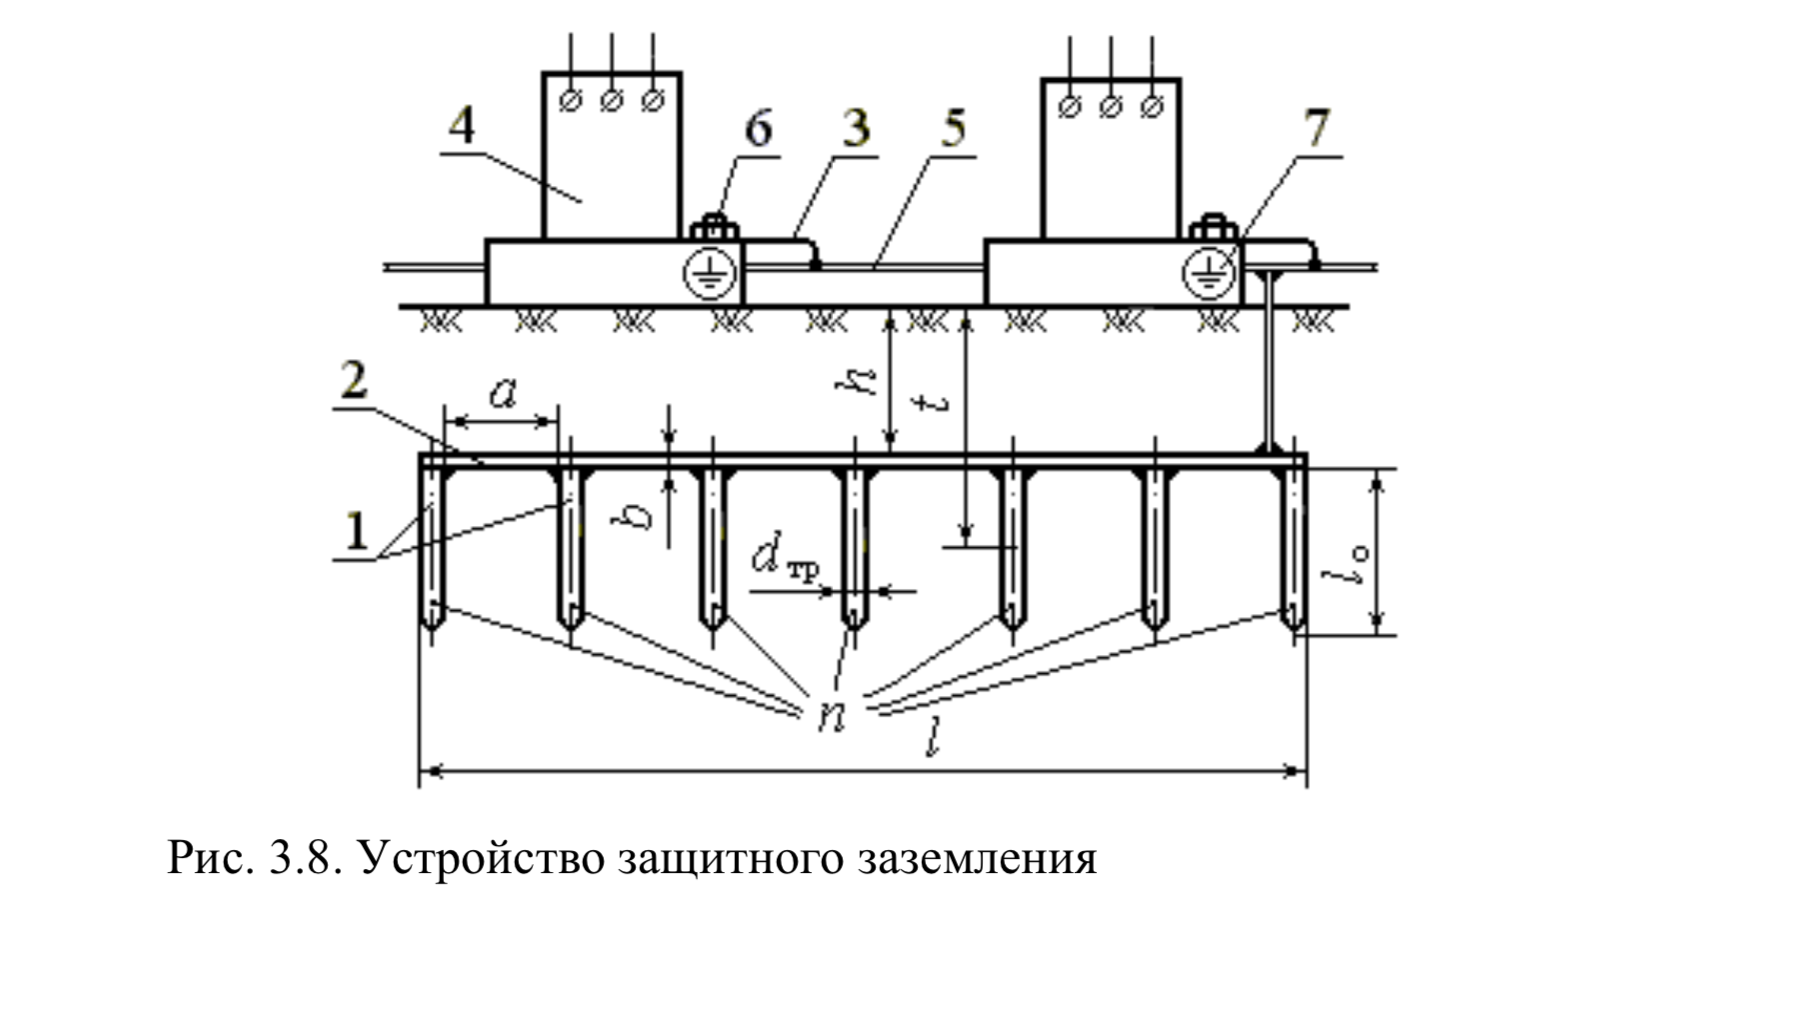
\includegraphics[width=\textwidth]{images/1.png}
\end{figure}

\begin{figure}
	\centering
	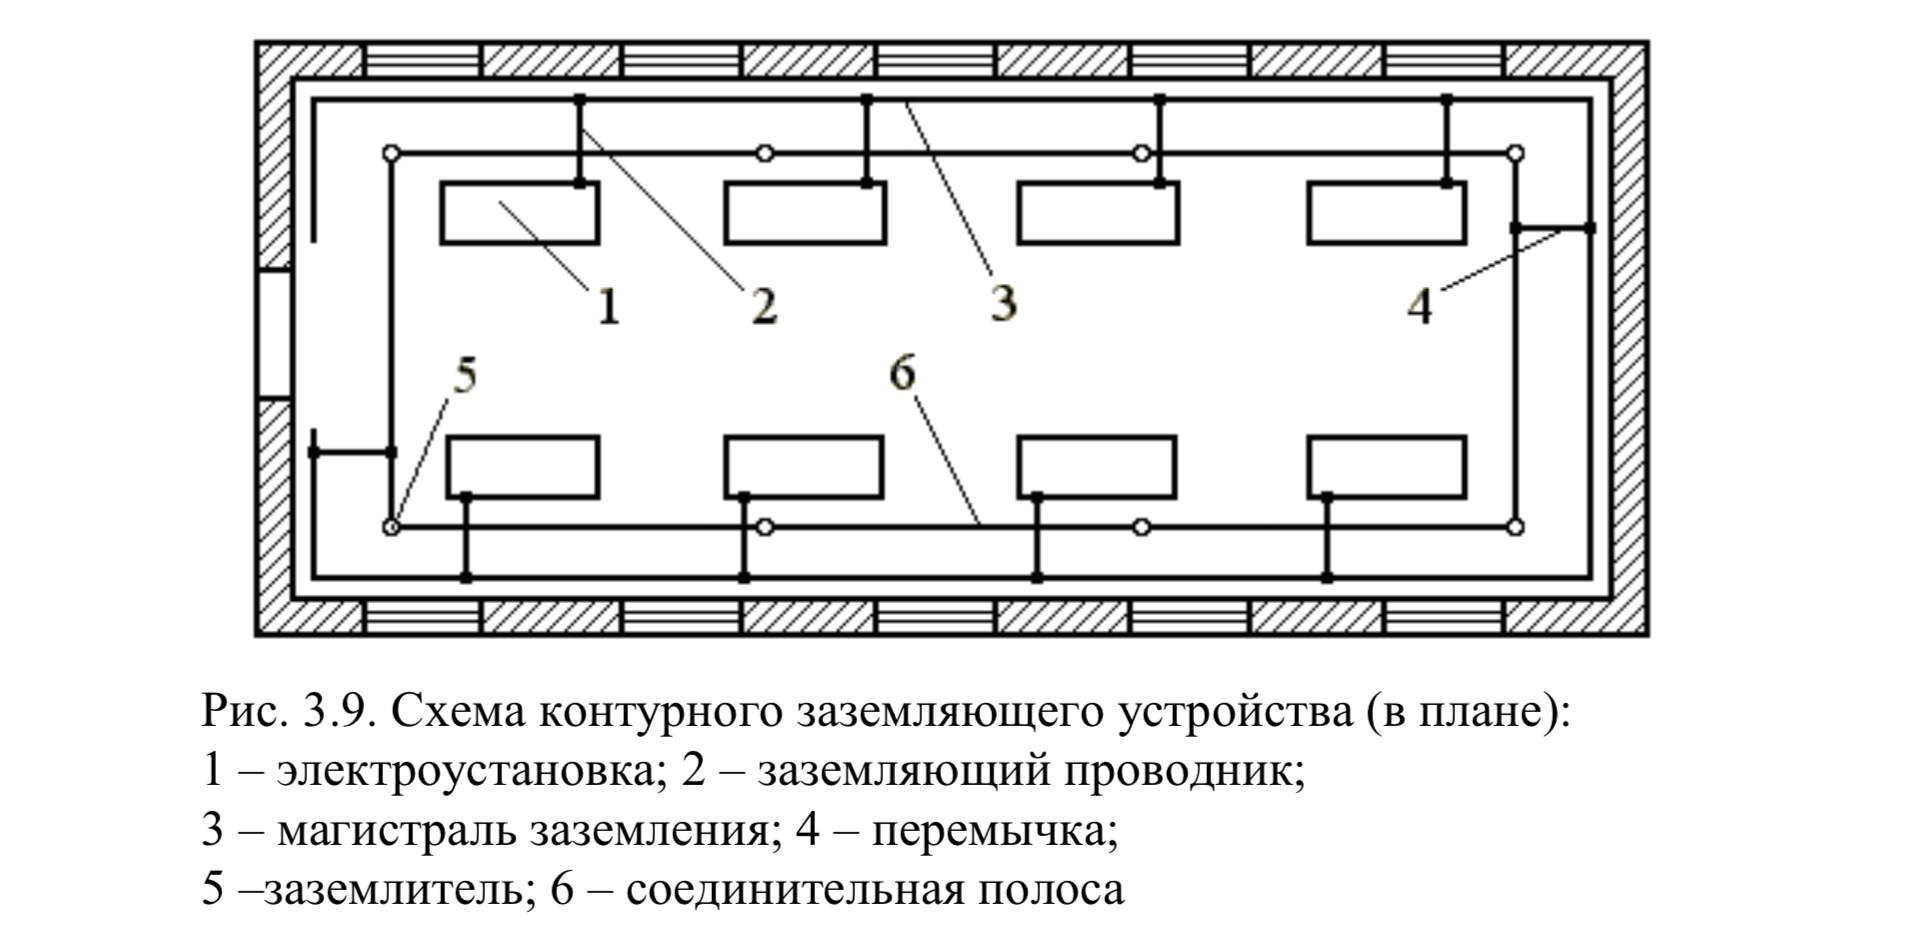
\includegraphics[width=\textwidth]{images/2.png}
\end{figure}
